\chapter{Analisi sperimentale}
\label{cap:analisi-sperimentale}

Nel corso di questo capitolo viene illustrata la fase di analisi sperimentale effettuata in questo lavoro, che mira a valutare i due algoritmi euristici proposti. Nella prima sezione viene illustrato il setup utilzzato per i test, successivamente viene fatta una panoramica sulle istanze utilizzate, ed infine si descrivono gli esperimenti e i risultati ottenuti.


%
%   SETUP
%
\section{Setup}
\label{sec:setup}

L'intera fase di analisi sperimentale, che comprende il caricamento dei dati, la loro manipolazione, l'elaborazione dei risultati e le analisi svolte, è stata effettuata utilizzando il linguaggio di programmazione Python \footnote{\url{https://www.python.org/}.} (versione \texttt{3.8.13}), integrato con alcune sue librerie:
\begin{itemize}
    \item Python-MIP \footnote{\url{https://www.python-mip.com/}.}: utilizzato per implementare ed eseguire i modelli di programmazione lineare illustrati precedentemente;
    \item NumPy \footnote{\url{https://numpy.org/}.}: utilizzata per rappresentare e manipolare i dati da gestire;
    \item Pandas \footnote{\url{https://pandas.pydata.org/}.}; utilizzata per effettuare analisi ed elaborazione dei dati:
    \item Matplotlib \footnote{\url{https://matplotlib.org}.}; utilizzata per generare i grafici.
\end{itemize}
Tutti i test sono stati eseguiti su una macchina con processore \texttt{Intel i7 8-core 4.00GHz} e \texttt{32GB} di memoria RAM, utilizzando il solutore Gurobi \footnote{\url{https://www.gurobi.com/}.} (versione \texttt{8.0.1 build v8.0.1rc0}) su sistema operativo Linux Ubuntu \footnote{\url{https://www.ubuntu-it.org/}.}, considerando un gap di ottimalità dello 0.1\% per determinare la soluzione ottima.


%
%   DATI UTILIZZATI
%
\section{Panoramica sui dati utilizzati}
\label{sec:dati-utilizzati}

Per condurre gli esperimenti, viene utilizzato il set di dati presentati nell'articolo \cite{assignment-patterns}, estratti da \cite{Barlacchi2015} e raffiguranti le richieste di traffico mobile nel mondo reale in un arco di due mesi su un'area geografica che si estende per oltre 2500 km$^2$. Come descritto, partendo dalla domanda vengono identificati 1419 AP (insieme $A$) e utilizzando le loro distanze euclidee si posizionano le 10 facility (insieme $K$), che compongono l'infrastruttura MEC. Le distanze di rete $m_{ik}$ e $l_{jk}$ vengono di conseguenza calcolate come distanze euclidee e arrotondate all'intero più vicino. Partendo da questa infrastruttura, sono state generate delle istanze in cui agli AP viene fornita una quantità di traffico casuale in modi diversi. 
In particolare, sono stati creati due dataset:
\begin{itemize}
    \item \textbf{Dataset A}: è sintetico e mette alla prova gli algoritmi dal punto di vista puramente computazionale;
    \item \textbf{Dataset B}: è realistico e riproduce le caratteristiche principali dei dati di partenza;
\end{itemize}
Tutte le istanze hanno un arco temporale di una giornata, e si considerano fascie composte da 12, 24, 48 e 96 time-slot. Per ogni dataset sono state create cinque diverse istanze per ogni numero di time-slot.


\subsection{Generazione dei dati energetici}

In ogni istanza precedentemente descritta, è necessario aggiungere i dati energetici $e^t_k$, che indicano per ogni time-slot, la quantità di energia prodotta da ciascuna facility. Ogni facility $k \in K$ possiede una certa potenza di produzione energetica indicata con $P_k$, che indica il suo tasso di conversione dell'irraggiamento solare in energia; in un contesto reale può essere considerato come una misura della quantità di pannelli fotovoltaici installati. Tale valore dipende dalla posizione geografica in cui si trova la facility, ed in particolare cresce all'aumentare della distanza dal centro dell'area considerata, con l'idea che andando verso l'esterno, lo spazio disponibile per piazzare i pannelli sia sempre maggiore. Il set di dati considerato riguarda l'area metropolitana della città di Milano, e di conseguenza il centro è definito dalla posizione geografica del Duomo di Milano \footnote{Coordinate UTM (WGS84) del Duomo di Milano: \texttt{E: 514962}, \texttt{N: 5034533}.}. La costante $P_k$ viene quindi definita come segue:
\begin{equation}
    P_k = \mu f(k)
\end{equation}
dove $\mu$ è il coefficiente che relaziona la distanza alla potenza produttiva, necessario per poter definire la quantità di energia complessivamente prodotta, mentre $f(k)$ è una misura della distanza di $k \in K$ dal punto centrale rispetto alle altre facility, e può essere definita in vari modi:
\begin{itemize}
    \item \textbf{costante}:
    \begin{equation}
        f_C(k) = 1
        \label{eq:fC}
    \end{equation}

    \item \textbf{lineare}:
    \begin{equation}
        f_L(k) = \frac{d(k)}{\underset{k \in K}{\max} ~ d(k)}
        \label{eq:fL}
    \end{equation}

    \item \textbf{quadratica}:
    \begin{equation}
        f_Q(k) = \frac{d(k)^2}{\underset{k \in K}{\max} ~ d(k)^2}
        \label{eq:fQ}
    \end{equation}

    \item \textbf{esponenziale}:
    \begin{equation}
        f_E(k) = \frac{e^{d(k)}}{e^{\underset{k \in K}{\max} ~ d(k)}}
        \label{eq:fE}
    \end{equation}
\end{itemize}
con $k \in K$ e dove $d(k)$ indica la distanza euclidea tra la facility $k$ e il centro dell'area.
La quantità $e^t_k$ di energia prodotta dalla facility $k \in K$ al tempo $t \in T$ è quindi data dalla radiazione solare a cui sono sottoposti i pannelli di $k$ nell'istante $t$, indicato con $r^r_k$, e dalla potenza di conversione della facility:
\begin{equation}
    e^t_k = P_k r^t_k.
\end{equation}
I dati riguardanti l'irraggiamento solare sono stati ottenuti dal Photovoltaic Geographical Information System~\footnote{\url{https://re.jrc.ec.europa.eu/pvg_tools/en/}.}, ossia un portale gestito dall'Unione Europea dal quale è possibile estrarre informazioni riguardo alla radiazione solare e le prestazioni del sistema fotovoltaico. In particolare, considerando le coordinate di ogni sito MEC, sono stati estratti i dati storici dell'anno 2020 con cadenza oraria: all'interno di ogni mese viene eseguita la media rispetto ai giorni, così da ottenere l'irraggiamento medio di ogni giorno di ogni mese.\\
I dati $c^t_k$, rappresentanti il prezzo che la facility $k \in K$ deve pagare per acquistare una unità di energia al tempo $t \in T$, vengono considerati fissi nel tempo:
\begin{align}
    &c^t_k = 1. && ~ \forall t \in T, ~ \forall k \in K
\end{align}
Pur producendo una diversa quantità di energia, tutte le facility hanno batterie con la stessa capienza, che viene fissata al valore medio di domanda da gestire in ogni facility e in ogni time-slot:
\begin{align}
    &G_k = \frac{\sum_{t \in T} \sum_{i \in A} d^t_i}{|T||K|}. && ~ \forall k \in K
\end{align}
Infine, resta da definire il valore del coefficiente $\mu$:
\begin{equation}
    \mu = \frac{\sum_{t \in T} \sum_{i \in A} d^t_i}{\sum_{t \in T} \sum_{k \in K} f(k)r^t_k}.
\end{equation}


%
%   TEST
%
\section{Test effettuati}
\label{sec:test}

La fase di test ha lo scopo di valutare le due euristiche proposte comparandole con il modello di assegnamento dinamico: viene quindi definito un set di istanze da calcolare, in modo da poter paragonare i risultati ottenuti e il tempo di calcolo necessario. Per poter avere una panoramica completa su tale confronto, è necessario utilizzare un insieme di istanze eterogeneo e considerare gli algoritmi in diverse configurazioni: i risultati ottenuti sono infatti fortemente influenzati dalle modalità utilizzate per dividere (euristica 1) e aggregare (euristica 2) i time-slot dell'istanza iniziale. In tutti i test eseguiti, i valori di $\alpha$, $\beta$ e $\gamma$ sono posti a $0.\bar{3}$. Successivamente viene fornita una panoramica sul set delle istanze e le configurazioni degli algoritmi.


%
%   SET DI ISTANZE
%
\subsection{Set di istanze}

Per testare gli algoritmi vengono utilizzate le istanze appartenenti al dataset B, così da poter valutare i risultati ottenuti su casi realistici ed osservare come si adattano alle variazioni di traffico nell'arco della giornata. Tra i vari formati, ci si concentra sulle istanze composte da 96 time-slot, che permettono di impegnarli maggiormente dal punto di vista computazionale e quindi valutarne al meglio le prestazioni. In ognuna di queste istanze vengono aggiunti i dati energetici, calcolati per ogni definizione della funzione $f$ (equazioni \ref{eq:fC}, \ref{eq:fL}, \ref{eq:fQ}, \ref{eq:fE}) e considerando l'irraggiamento nei mesi di dicembre, settembre e luglio, che rappresentano rispettivamente in media, il minore, medio e maggiore. In conclusione, il set sarà quindi composto da: 5 (istanze da 96 time-slot) $\times$ 4 (definizioni di $f$) $\times$ 3 (mesi irraggiamento) = 60 istanze.


%
%   CONFIGURAZIONI
%
\subsection{Configurazione degli algoritmi}

Entrambi gli algoritmi euristici considerati presentano un certo grado di libertà, dato dal modo in cui viene rispettivamente frammentata e semplificata l'istanza da computare. Tale scelta condiziona i tempi di calcolo e il risultato ottenuto, e di conseguenza per avere una panoramica il più completa possibile sul loro funzionamento, si testano diverse strategie. Per ottenere una migliore chiarezza espositiva, ogni configurazione viene identificata da un nome del tipo \texttt{E1\_CONFIG\_ALTRO}, dove la prima parte indica l'euristica, la seconda la configurazione e il resto varie specifiche.

\subsubsection{Euristica 1}

Le strategie considerate per suddividere l'istanza iniziale in sottoistanze sono le seguenti:
\begin{itemize}
    \item \texttt{E1\_UGUALE\_T}: Effettuare la suddivisione facendo in modo che ogni sottoistanza abbia la stessa quantità di domanda complessiva da gestire, ottenendo sottoistanze ristrette quando si considerano fascie orarie con ampio uso della rete (generalmente durante il giorno) ed istanze più grandi quando l'uso è limitato (di solito durante la notte). In genere, non è possibile effettuare la suddivisione ottenendo esattamente in ciascuna la stessa domanda, e per questo si tenta di minimizzarne la loro differenza tramite il modello di ottimizzazione descritto nella \autoref{sec:framm-equals}, dove il vettore in input rappresenta l'arco temporale, ed ogni elemento contiene la quantità di domanda complessiva da gestire in quel time-slot. I blocchi restituiti indicano come deve essere eseguita la frammentazione, infatti per ciascuno viene creata una sottoistanza.

    \item \texttt{E1\_LAD-LSD\_T}: Suddividere l'istanza in modo da minimizzare la differenza di domanda all'interno di ogni sottoistanza, ottenendo quindi in ciascuna time-slot il più omogenei possibile tra loro. L'implementazione viene effettuata attraverso il modello di ottimizzazione presente nella \autoref{sec:framm-omogenei}, dove il vettore in input, come nel caso precedente, è formato dalla quantità di traffico complessiva presente in ogni time-slot, e i blocchi in output descrivono in che modo segmentare l'arco temporale. Per definire la differenza $d_{ij}$ tra due elementi $i$ e $j$, vengono considerati due modelli:
    \begin{itemize}
        \item Least Absolute Deviation (LAD): $d_{ij} = |q_i - q_j|$;
        \item Least Squared Difference (LSD): $d_{ij} = (q_i - q_j)^2$.
    \end{itemize}
\end{itemize}
In entrambi i casi si esamina la suddivisione in 12, 24 e 48 sottoistanze, e la \texttt{T} nel nome va sostituita con tale valore.

Vengono inoltre considerati i due casi estremi:
\begin{itemize}
    \item \texttt{E1\_MIGRAZIONI\_0}: La suddivisione viene effettuata in tante parti quanti sono i time-slot che compongono l'istanza, ottenendo sottoistanze formate da un singolo istante temporale. In questo modo le istanze vengono risolte senza considerare i costi di migrazione da pagare, che si suppongono essere 0, e di conseguenza gli assegnamenti avvantaggeranno la latenza e la gestione energetica ottenute. Avendo grandezza unitaria, le sottoistanze vengono risolte utilizzando il modello di assegnamento descritto nella \autoref{sec:modello-singolo-slot}, creato ad hoc per questa tipologia.

    \item \texttt{E1\_MIGRAZIONI\_INF}: Utilizzare l'istanza completa senza effettuare suddivisioni. In questo caso, nell'eseguire l'ottimizzazione si considera di pagare un costo infinito a seguito di ogni switch: le orchestrazioni diventeranno quindi inefficienti e ogni AP rimarrà associato alla stessa facility per tutto l'arco temporale, a discapito della latenza e dell'efficienza energetica. In questo modo il problema perde la caratteristica della dinamicità. Da notare come, trattandosi di una singola istanza, non sia necessario utilizzare l'\autoref{alg:euristica-semplificazione-modello}, ma sia sufficiente il modello di assegnamento statico (\autoref{sec:modello-statico}).
\end{itemize}

\subsubsection{Euristica 2}

In questo caso viene considerata una sola strategia per semplificare l'istanza.
\begin{itemize}
    \item \texttt{E2\_LAD-LSD\_T}: L'istanza iniziale viene frammentata minimizzando la differenza di domanda all'interno di ogni frammento allo stesso modo delle configurazioni \texttt{E1\_LAD\_T} e \texttt{E1\_LSD\_T}, e per ciascuno viene scelto come rappresentante il time-slot mediano utilizzato nell'effettuare l'ottimizzazione. Anche in questo caso vengono considerate suddivisioni da 12, 24 e 48 time-slot, e la \texttt{T} va sostituita con tale valore.
\end{itemize}


%
%   RISULTATI
%
\section{Risultati ottenuti}
\label{sec:risultati}

In questa sezione vengono mostrati ed analizzati i risultati ottenuti dalle computazioni.

\subsection{Analisi generale}

Nella \hyperref[tab:medie-iniziali]{tabella 1} vengono presentati i valori e i tempi di esecuzione medi dei risultati ottenuti per ogni configurazione, dove con \texttt{MODELLO\_DINAMICO} viene indicato il modello di assegnamento dinamico (\autoref{sec:modello-dinamico}). La prima colonna indica la configurazione considerata, nella seconda è presente la media dei valori della funzione obbietto del modello di assegnamento dinamico (\hyperref[eq:dinamico-obj]{equazione 3.1.1}) calcolata sui risultati ottenuti, ed infine è indicata la media dei tempi di esecuzione, nel formato: ore, minuti, secondi e millisecondi. Osservando la tabella, si nota come l'uso degli algoritmi euristici apporta una grossa riduzione del tempo di calcolo necessario a risolvere le istanze del set considerato, infatti partendo dal \texttt{MODELLO\_DINAMICO} che impiega in media più di mezzora, le configurazioni della seconda euristica necessitano di pochi minuti, mentre quelle della prima alcuni secondi.

\begin{table}[t]
    \centering
    \scalebox{0.85}{
        \begin{tabular}{lrl}
            \toprule
            {} &  valore obbiettivo & tempo di esecuzione \\
            configurazione             &                    &                     \\
            \midrule
            \texttt{MODELLO\_DINAMICO}  &       1.212566e+11 &        00:36:35.896 \\
            \texttt{E1\_LAD\_12}         &       1.253934e+11 &        00:00:04.780 \\
            \texttt{E1\_LAD\_24}         &       1.245708e+11 &        00:00:05.213 \\
            \texttt{E1\_LAD\_48}         &       1.252199e+11 &        00:00:06.583 \\
            \texttt{E1\_LSD\_12}         &       1.251684e+11 &        00:00:04.658 \\
            \texttt{E1\_LSD\_24}         &       1.246440e+11 &        00:00:05.304 \\
            \texttt{E1\_LSD\_48}         &       1.258861e+11 &        00:00:06.509 \\
            \texttt{E1\_MIGRAZIONI\_0}   &       1.261016e+11 &        00:00:09.125 \\
            \texttt{E1\_MIGRAZIONI\_INF} &       1.422782e+11 &        00:00:21.114 \\
            \texttt{E1\_UGUALE\_12}      &       1.252572e+11 &        00:00:05.349 \\
            \texttt{E1\_UGUALE\_24}      &       1.257407e+11 &        00:00:05.510 \\
            \texttt{E1\_UGUALE\_48}      &       1.261911e+11 &        00:00:07.255 \\
            \texttt{E2\_LAD\_12}         &       1.225128e+11 &        00:00:47.196 \\
            \texttt{E2\_LAD\_24}         &       1.258975e+11 &        00:02:13.861 \\
            \texttt{E2\_LAD\_48}         &       1.362601e+11 &        00:06:47.127 \\
            \texttt{E2\_LSD\_12}         &       1.251709e+11 &        00:00:48.317 \\
            \texttt{E2\_LSD\_24}         &       1.254649e+11 &        00:02:39.567 \\
            \texttt{E2\_LSD\_48}         &       1.367933e+11 &        00:07:56.186 \\
            \bottomrule
        \end{tabular}
    }
    \caption{Valori medi dei risultati ottenuti.}
    \label{tab:medie-iniziali}
\end{table}

Nella \hyperref[graf:peggioramento-perc]{figura 3} viene mostrato il peggioramento medio percentuale dei risultati ottenuti da ciascuna configurazione rispetto all'ottimo. Si nota immadiatamente come il range di peggioramento sia tra l'1\% ed il 17.5\% circa, e come la configurazione \texttt{E2\_LAD\_12} generi i risultati migliori, a differenza della \texttt{E1\_MIGRAZIONI\_INF} che ottiene in media i peggiori. Le restanti hanno tutte un peggioramento che varia tra il 2.5\% ed il 4\%, a differenza delle configurazioni da 48 time-slot dell'euristica 2, che peggiorano l'ottimo di circa il 12.5\%.

\begin{figure}[H]
    \centering
    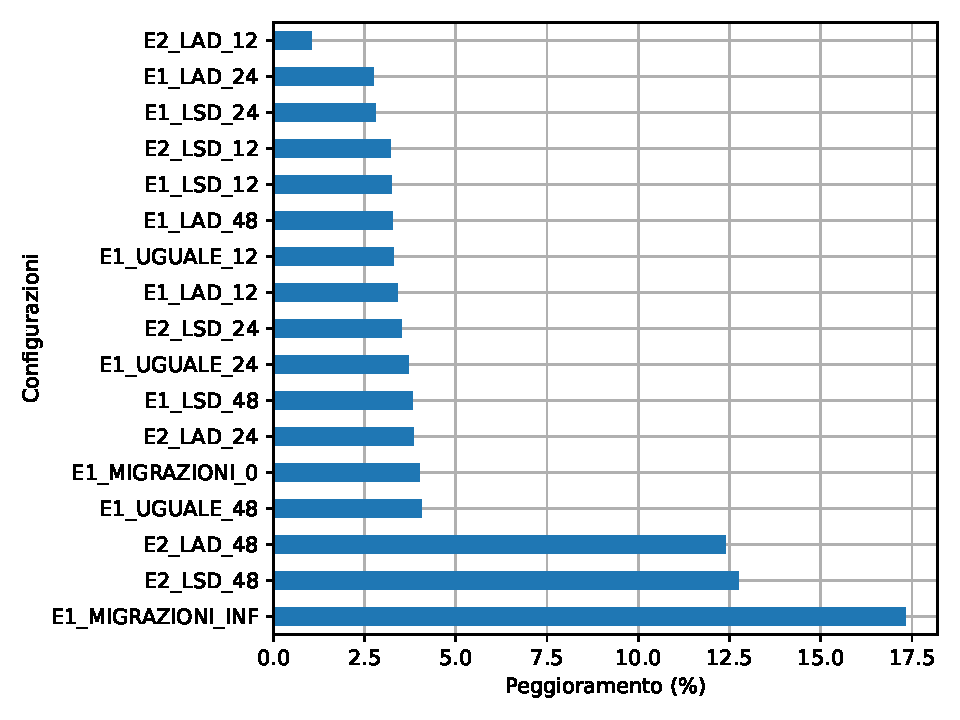
\includegraphics[scale=0.75]{img/grafico-peggioramento-percentuale.pdf}
    \caption{Peggioramento percentuale delle configurazioni rispetto ai valori ottimi.}
    \label{graf:peggioramento-perc}
\end{figure}

%
%   EURISTICA 1
%
\subsection{Risultati euristica 1}

\begin{figure}[H]
    \centering
    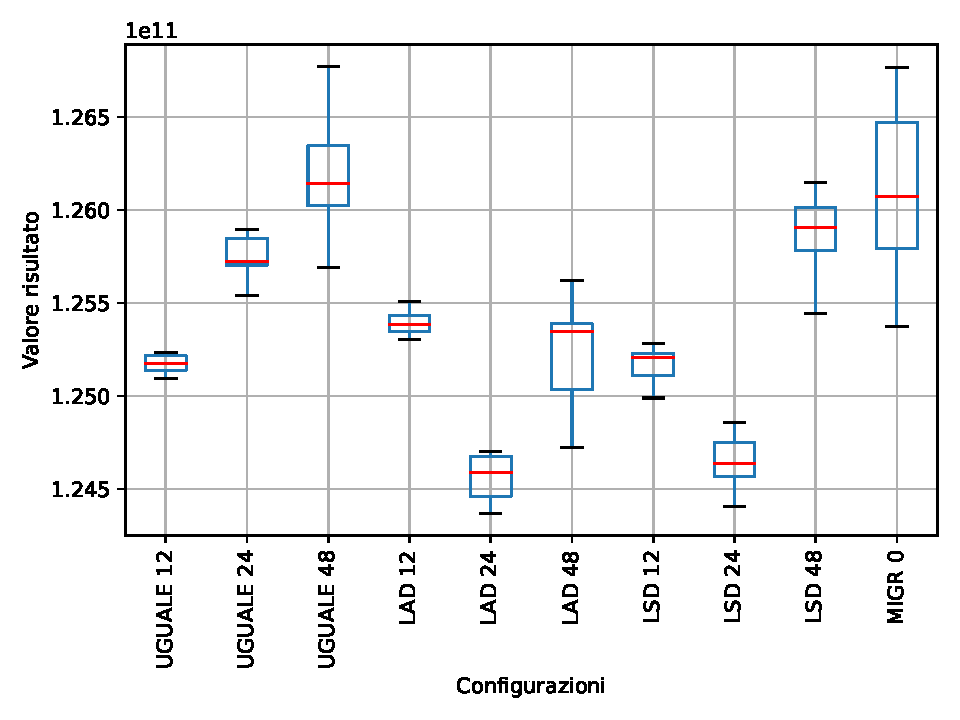
\includegraphics[scale=0.70]{img/grafico-e1-valore.pdf}
    \caption{Distribuzione dei risultati ottenuti usando l'euristica 1.}
    \label{graf:e1-valore-range}
\end{figure}

\begin{figure}[H]
    \centering
    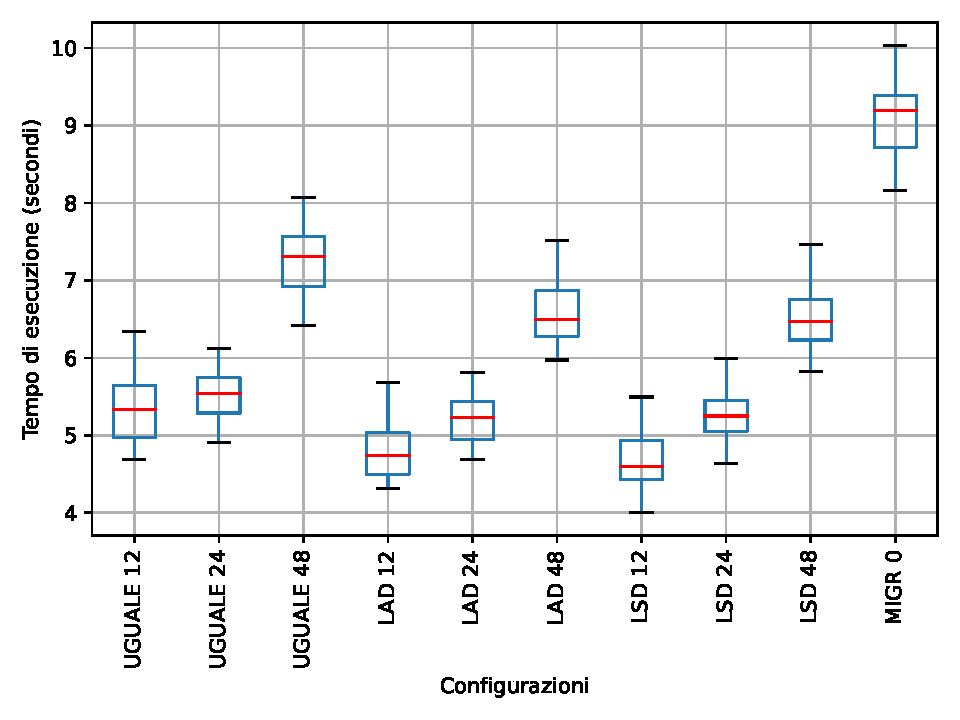
\includegraphics[scale=0.70]{img/grafico-e1-tempo.pdf}
    \caption{Distribuzione dei tempi di calcolo ottenuti usando l'euristica 1.}
    \label{graf:e1-tempo-range}
\end{figure}

\begin{figure}[H]
    \centering
    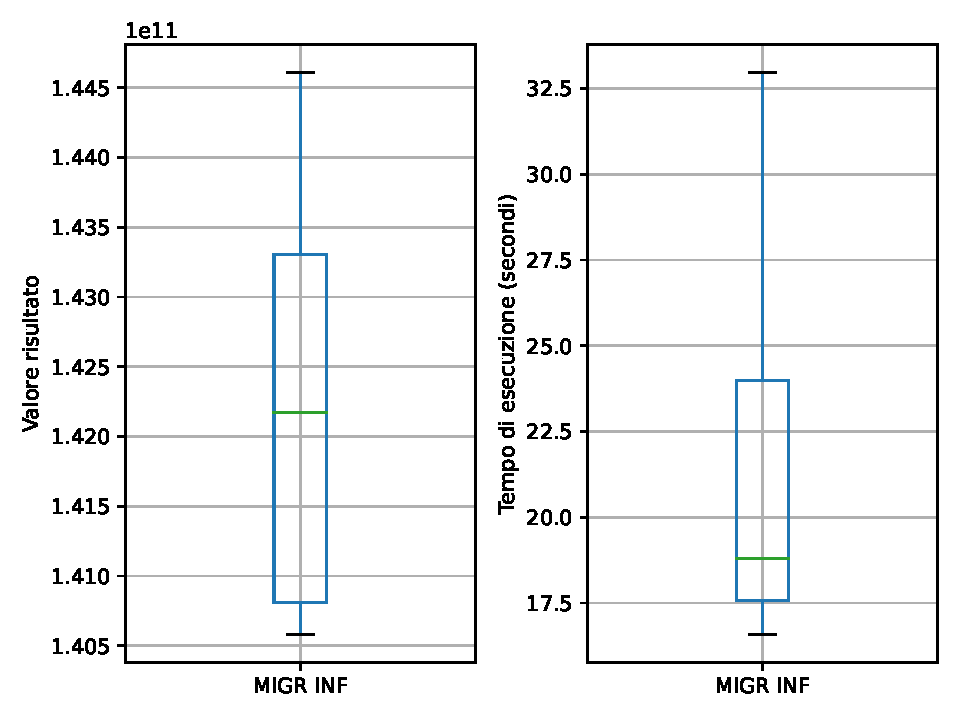
\includegraphics[scale=0.70]{img/grafico-e1-inf.pdf}
    \caption{Distribuzione dei risultati e dei tempi di calcolo ottenuti usando la configurazione \texttt{MIGRAZIONI\_INF}.}
    \label{graf:e1-inf}
\end{figure}

Una panoramica completa sui risultati ottenuti utilizzando le configurazioni della prima euristica, è mostrata nelle figure \ref{graf:e1-valore-range} e \ref{graf:e1-tempo-range}, che illustrano la distribuzione dei valori obbiettivo risultanti e dei tempi di calcolo impiegati. In tali figure non sono presenti i dati riguardanti la configurazione con migrazioni a costo infinito (\texttt{E1\_MIGRAZIONI\_INF}), dato che avendo una scala diversa rispetto agli altri valori, si sarebbero ottenuti grafici più compressi, e di conseguenza le sue distribuzioni sono mostrate nella \hyperref[graf:e1-inf]{figura 6}.

Osservando le distribuzioni dei valori risultanti, sembra chiaro come nei casi \texttt{LAD} e \texttt{LSD} suddividere l'istanza in 24 parti porti a risultati migliori rispetto alla suddivisione in 12 o 24, mentre nella configurazione \texttt{UGUALE} conviene dividere in 12. In generale, osservando il confronto tra i due casi estremi (\texttt{MIGRAZIONI\_0} e \texttt{MIGRAZIONI\_INF}), si nota come l'algoritmo tragga più beneficio nell'effettuare molte suddivisioni rispetto a non farne nessuna: questo evidenzia come la latenza e la gestione dell'energia abbiano un impatto molto maggiore rispetto al costo da pagare per le migrazioni.


%
%   EURISTICA 2
%
\subsection{Risultati euristica 2}

\begin{figure}[H]
    \centering
    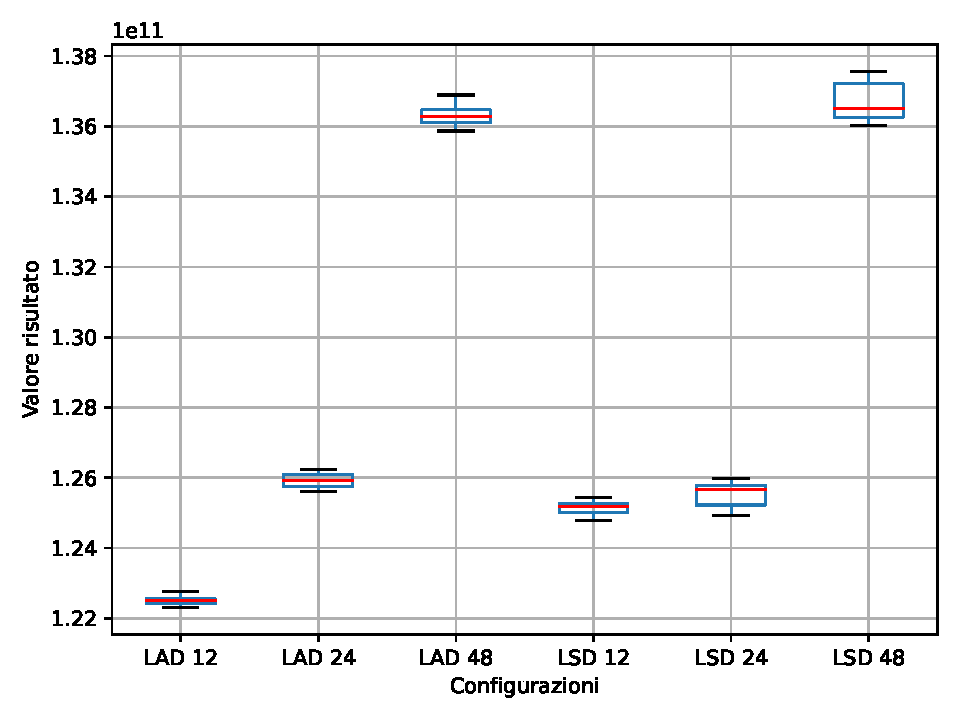
\includegraphics[scale=0.70]{img/grafico-e2-valore.pdf}
    \caption{Distribuzione dei risultati ottenuti usando l'euristica 2.}
    \label{graf:e2-valore-range}
\end{figure}

\begin{figure}[H]
    \centering
    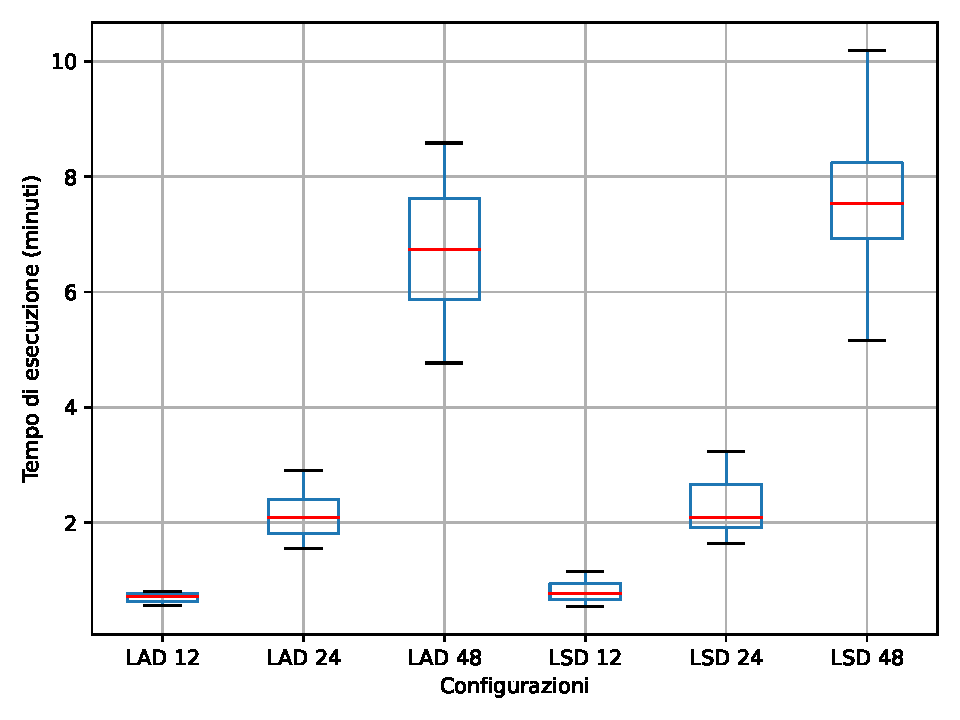
\includegraphics[scale=0.70]{img/grafico-e2-tempo.pdf}
    \caption{Distribuzione dei tempi di calcolo ottenuti usando l'euristica 2.}
    \label{graf:e2-tempo-range}
\end{figure}

Come nell'analisi precedente, vengono rappresentati i grafici rappresentanti le distribuzioni dei valori ottenuti (\hyperref[graf:e2-valore-range]{figura 7}) e dei tempi di esecuzione risultanti (\hyperref[graf:e2-tempo-range]{figura~8}).

Nel grafico riguardante i valori dei risultati, viene chiaramente mostrato come effettuare la semplificazione in istanze piccole sia più vantaggioso rispetto a quelle più grandi. I tempi di esecuzione sottolineano invece la complessità combinatoria del modello di assegnamento dinamico, utilizzato per risolvere le sottoistanze: al crescere nel numero di fascie temporali, il tempo di esecuzione aumenta esponenzialmente. Confrontando le due metriche, è chiaro come il metodo utilizzato per frammentare l'istanza sia molto meno determinante rispetto alla dimensione dell'istanza semplificata.
\begin{figure}[H]
    \centering
    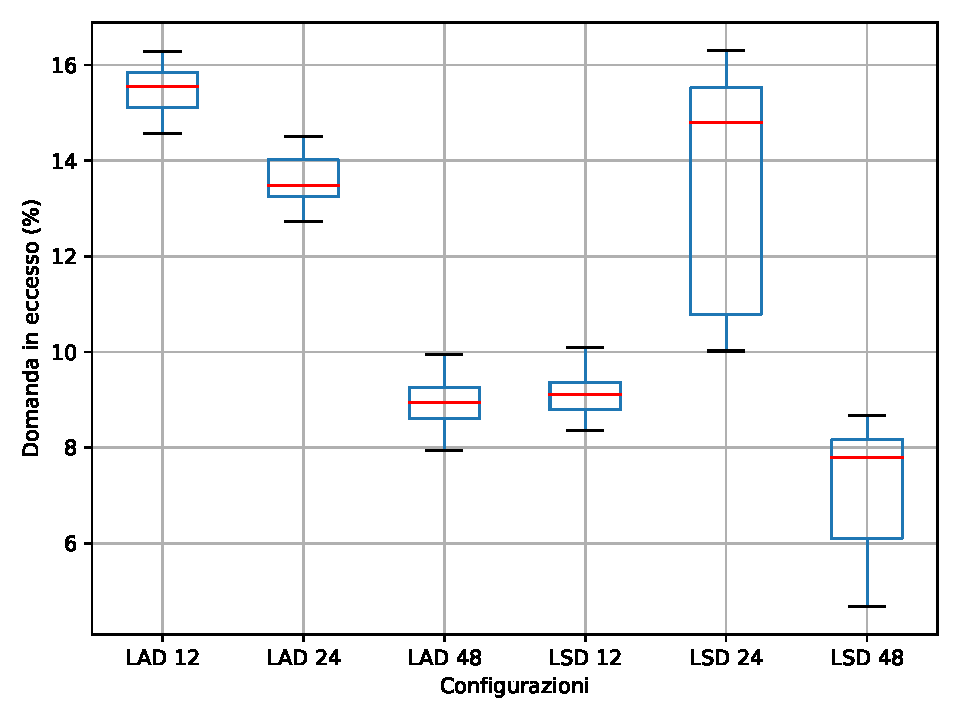
\includegraphics[scale=0.70]{img/grafico-e2-eccesso.pdf}
    \caption{Distribuzione della quantità percentuale di domanda in eccesso assegnata alle facility in ogni configurazione.}
    \label{graf:e2-eccesso-range}
\end{figure}
Per ottenere un'analisi completa di questa euristica, è necessario calcolare e valutare la quantità di domanda che eccede dalla capienza delle facility. Tale valore è dato dalla somma della domanda in eccesso in ogni facility e in ogni istante temporale:
\begin{equation}
    \sum_{t \in T} \sum_{k \in K} \max\{0, v^t_k - C_k\}.
\end{equation}
Nella \hyperref[graf:e2-eccesso-range]{figura 9} viene mostrata la distribuzione percentuale di tale quantità.
